% !TeX spellcheck = en_GB

\documentclass[aspectratio=169,]{beamer}

\usepackage[utf8]{inputenc}
\usepackage[english]{babel}
\usepackage[percent]{overpic}
%\usepackage{appendixnumberbeamer}

\usepackage{tikz}
\usetikzlibrary{shapes,arrows,positioning,calc}

\tikzstyle{startstop} = [ellipse, draw, fill=bg, text=structure, text width=3em, text badly centered, inner sep=0pt]
\tikzstyle{block} = [rectangle, draw, fill=bg, text=structure, text width=5em, text centered]
\tikzstyle{decision} = [diamond, aspect=3, draw, fill=bg, text=structure, text width=3em, text badly centered, inner sep=0pt]
\tikzstyle{input} = [trapezium, draw, fill=bg, text=structure, text width=5em, text centered, trapezium right angle=120]
\tikzstyle{output} = [trapezium, draw, fill=bg, text=structure, text width=5em, text centered, trapezium right angle=120]

\tikzstyle{line} = [draw, -latex']

%\usepackage{xcolor}
\usepackage{listings}

\lstdefinestyle{pseudo}{
	backgroundcolor=\color{bg},
	keywordstyle=\color{alert},
	numberstyle=\tiny\color{fg!50},
	numbers=left,
	%commentstyle=\color{mGreen},
	%stringstyle=\color{mPurple},
    mathescape=true,
	basicstyle=\scriptsize,
    keywords={input,output,begin,end,if,then,else,while,do,for,each,return}
	%tabsize=4,
	%breakatwhitespace=false,
	%breaklines=true,
	%captionpos=b,
	%keepspaces=true,
	%numbersep=5pt,
	%showspaces=false,
	%showstringspaces=false,
	%showtabs=false,
	%language=C
}

\usepackage{minted}


\usetheme[titleformat=smallcaps, numbering=fraction, background=light, progressbar=frametitle]{metropolis}

\title{Digital Technology}
\subtitle{Introduction to Python programming}

\author{Stefano Cereda\\
		stefano.cereda@polimi.it
	}
\date{17/03/2020}
\institute[PoliMi]{Politecnico Milano}
\logo{
\includegraphics[width=15mm]{../logopolimi}}

\setbeamercovered{invisible}

\makeindex

\begin{document}
\begin{frame}
	\maketitle
\end{frame}

\begin{frame}{Python programming}
    Computer Programming is the process of designing an \alert{algorithm} and implementing it with a
    \alert{programming language} so to obtain an executable computer program to accomplish a specific computing result.

    We first need to apply \emph{problem solving} skills to design an algorithm, then we will define the solution
    clearly and accurately in a programming language.
\end{frame}

\begin{frame}{Algorithm}
    An algorithm is a \alert{finite sequence of well-defined, unambiguous and computer-implementable instructions}.

    ``Draw a nice painting'' is \emph{not} an algorithm.
    ``Multiply two numbers and subtract 3 to the results'' is an algorithm.

    Typically, an algorithm solves a class of problems or performs a computation.
\end{frame}

\begin{frame}{Algorithm definition}
    We can describe an algorithms with different languages: flowcharts, pseudocode, programming languages.
\end{frame}

\begin{frame}{Defining an algorithm: flowcharts}
    \begin{tikzpicture}[auto, node distance=0.75cm]
		\node [startstop] (start) {Begin};
		\node [input, below = of start] (in) {Input};
		\node [block, below = of in] (increment) {Do};
		\node [decision, below = of increment] (decision) {?};
		\node [output, below left = of decision] (outpos) {Output};
		\node [output, below right = of decision] (outneg) {Output};
		\node [startstop, below = 1.5 of decision] (stop) {End};

		\path [line] (start) -- (in);
		\path [line] (in) -- (increment);
		\path [line] (increment) -- (decision);
		\path [line] (decision) -| node [near end] {true} (outpos);
		\path [line] (decision) -| node [near end] {false} (outneg);
		\path [line] (outpos) -- (stop);
		\path [line] (outneg) -- (stop);

		\node [right = 1.5 of start] {Start block};
		\node [right = 1.5 of in] {Data input block};
		\node [right = 1.5 of increment] {Execution block};
        \node [right = 1.5 of decision] {Condition block (selection/iteration)};
		\node [right = .5 of outneg] {Data output block};
		\node [right = 1.5 of stop] {Finish block};
		\end{tikzpicture}
\end{frame}

\begin{frame}{Flowchart example: the friendship algorithm}
    \centering
    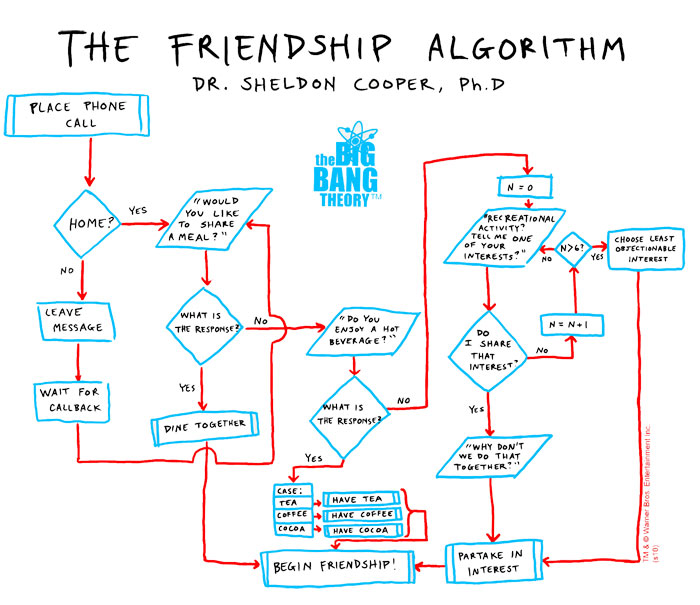
\includegraphics[height=\textheight]{block_sheldon.png}
\end{frame}

\begin{frame}[fragile]{Pseudocode example: Euclid's algorithm for GCD}
    \begin{lstlisting}[style=pseudo, linewidth=7cm]
input: Two integer numbers A and B.
output: The greatest common divisor of A and B.
begin
A = |A|
B = |B|

while B $\neq$ 0 do:
    if A > B then:
        A $\leftarrow$ A - B
    else:
        B $\leftarrow$ B - A
return A
end
    \end{lstlisting}
\end{frame}

\begin{frame}{Problem solving}
    To solve a problem, we will use the following steps:
    \begin{enumerate}
        \item{Problem comprehension}
        \item{Step-wise refinement}
        \item{Solution writing}
        \item{Solution testing}
    \end{enumerate}
\end{frame}

\begin{frame}[fragile]{Defining an algorithm: find the maximum}
    Find the maximum in a list of numbers L=[1,2,3,2,1,4]

    \pause
    We have an easy way to find the maximum between two numbers:
    \begin{lstlisting}[style=pseudo, linewidth=7cm]
input: two numbers A and B
output: the greatest number between A and B
begin:
if A > B then:
    return A
else:
    return B
end
    \end{lstlisting}
    \pause
    We can find $\max(L)$ as: $\max(4, \max(1,2,3,2,1))$ = $\max(4, \max(1, \max(1,2,3,2)))$ = $\dots$
    = $\max(4, \max(1, \max(2, \max(3, \max(2, 1)))))$
\end{frame}

\begin{frame}[fragile]{Algorithm to find the maximum}
    \begin{minipage}{0.49\textwidth}
        \begin{lstlisting}[style=pseudo, linewidth=7cm]
input: A list of numbers L.
output: The largest number in the list L.
begin
if L is empty:
    return Null

max $\leftarrow$ L[0]
for each number in L do
    if number $>$ max then
        max $\leftarrow$ number
return max
end
        \end{lstlisting}
    \end{minipage}
    \begin{minipage}{0.49\textwidth}
        \centering
        \resizebox{!}{6cm}{
        \begin{tikzpicture}[auto, node distance=1cm]
            \node [startstop] (start) {Begin};
            \node [input, below = of start] (in) {Read L};
            \node [decision, below = of in] (empty) {L is empty?};
            \node [output, right = of empty] (null) {Null};
            \node [block, below = of empty] (init) {max=L[0], i=1};
            \node [decision, below = of init] (while) {i < |L|?};
            \node [decision, below = of while] (check) {L[i] > max?};
            \node [block, right = of check] (swap) {max = L[i]};
            \node [block, below = of check] (increment) {i = i+1};
            \node [output, right = of while] (output) {max};
            \node [startstop, right = of output] (end) {End};

            \path [line] (start) -- (in);
            \path [line] (in) -- (empty);
            \path [line] (empty) -- (null);
            \path [line] (empty) -- (init);
            \path [line] (init) -- (while);
            \path [line] (while) -- node [near start] {true} (check);
            \path [line] (while) -- node [near start] {false} (output);
            \path [line] (check) -- node [near start] {true} (swap);
            \path [line] (check) -- node [near start] {false} (increment);
            \path [line] (swap) |- (increment);
            \path [line] (output) -- (end);
            \path [line] (null) -| (end);
            \path [line] (increment) -- ($ (increment) + (-2, 0)$) |- (while);
            %\path [line] (start) -- (in);
            %\path [line] (in) -- (increment);
            %\path [line] (increment) -- (decision);
            %\path [line] (decision) -| node [near end] {true} (outpos);
            %\path [line] (decision) -| node [near end] {false} (outneg);
            %\path [line] (outpos) -- (stop);
            %\path [line] (outneg) -- (stop);

            %\node [right = 1.5 of start] {Start block};
            %\node [right = 1.5 of in] {Data input block};
            %\node [right = 1.5 of increment] {Execution block};
            %\node [right = 1.5 of decision] {Condition block (selection/iteration)};
            %\node [right = .5 of outneg] {Data output block};
            %\node [right = 1.5 of stop] {Finish block};
        \end{tikzpicture}
    }
    \end{minipage}
\end{frame}

\begin{frame}{Prime number}
    Design an algorithm to check whether a number $N$ is a prime number.
    \pause
    \begin{itemize}[<+->]
        \item A number is prime if it can be divided only by 1 and itself.
        \item We should check all the numbers between 2 and $\sqrt{N}$ looking for divisor of $N$.
        \item A number $D$ is a divisor of $N$ if $N \% D = 0$, where \% is the modulo operation (remainder of integer
            division)
    \end{itemize}
\end{frame}

\begin{frame}[fragile]{Pseudocode for pime number}
    \begin{lstlisting}[style=pseudo, linewidth=7cm]
input: A number N.
output: A boolean value indicating whether N is prime or not.
begin
for each natural number D between 2 and $\sqrt{N}$:
    if N % D = 0 then:
        return False
return True
    \end{lstlisting}
    Pay attention to the indentation of return True
\end{frame}


\begin{frame}{Python}
    Python is an \alert{interpreted, high-level, general-purpose} programming language created in 1991.

    \pause
    Nice, but what does it mean?

    \pause
    \begin{itemize}[<+->]
        \item Interpreted = instructions are executed directly, without previously translating the program in
            machine-language.
        \item High level = strong abstraction from computer details.
        \item  General-purpose = designed to write software for the widest variety of application domains
    \end{itemize}
\end{frame}

\begin{frame}{Python REPL}
    We can use the Python interpreter in two ways: immediate mode and script mode.

    In the immediate mode, you type an expression and the interpreter immediately shows the result.
    This is called \alert{REPL}, for Read, Evaluate, Print Loop.

    \centering
    \begin{overpic}[width=\textwidth]{python_repl}
        \put (12,7) {\alert{$\leftarrow$ You type an expression}}
        \put (5,4) {\alert{$\leftarrow$ The interpreter reads and evaluates it and then replies}}
        \put (8,1) {\alert{$\leftarrow$ We are ready for another loop}}
    \end{overpic}
\end{frame}

\begin{frame}{Python scripts}
    In the script mode, you write a program in a file and use the interpreter to execute the contents of the file.
    Such a file is called a script.
    Scripts have the advantage that they can be saved to disk, printed, and so on.

    A script is just a text file, so you can use whichever editor you prefer to write i,
    I will use Vim\footnote{\url{https://en.wikipedia.org/wiki/Editor_war}}

    You can try PyCharm\footnote{\url{https://www.jetbrains.com/pycharm/}}, which is  a nice IDE available for
    GNU/Linux, Windows and Mac.
    You will also need to install Python\footnote{\url{https://www.python.org/downloads/}}.
    Make sure you are using Python 3 and not Python 2.
\end{frame}

\begin{frame}{Online Python}
    If you do not want to install software on your PC, you can use an online environment: \url{https://repl.it}.
    However, keep in mind that the it comes with limited resources.

    \centering
    \begin{overpic}[width=0.8\textwidth]{repl.png}
        \put (0,30) {\alert{File Manager}}
        \put (25,25) {\alert{Text Editor}}
        \put (65,30) {\alert{Python Interpreter}}
    \end{overpic}
\end{frame}

\begin{frame}[fragile]{Hello world!}
    Let's create our first python program:
    \begin{minted}{python}
print("Hello world!")
    \end{minted}
    Test the code in immediate mode and in script mode.
\end{frame}


\begin{frame}{Python variables}
    \begin{itemize}[<+->]
        \item A \emph{variable} is a memory location where you can store data.
        \item Differently from other languages, you do not need to explicitly declare a variable
        \item Every data value has a \emph{type} (e.g., number, list, character, string, \ldots)
        \item Python uses a \emph{dynamic} type system, so a variable can change its type over time
    \end{itemize}
\end{frame}

\begin{frame}[fragile]{Python variables: examples}
    \begin{minted}[fontsize=\scriptsize]{python}
# This is a comment (= text ignored by python)
# Declare and initialize an integer variable
a = 0
# You can check the type of a variable with:
type(a)
# Now a string (= sequence of character)
a = 'Hello world!'
type(a)
# You can assign to a variable the result of an operation
a = 1
b = 2
c = a+b
type(c)
    \end{minted}
Run the code in Python REPL
\end{frame}

\begin{frame}[fragile]{Python output}
    You can use the \alert{print} instruction to show the value of a variable:
    \begin{minted}[fontsize=\scriptsize]{python}
print(4)
a=2
print(a)
    \end{minted}
    This code will print 4 and 2 on two different lines.

    You can also combine a string with a variable:
    \begin{minted}[fontsize=\scriptsize]{python}
a = 42
print('The answer you are looking for is ', a)
    \end{minted}
    This code will print ``The answer you are looking for is 42''
\end{frame}

\begin{frame}[fragile]{Python input}
    You can use the \alert{input} instruction to read some values:
    \begin{minted}[fontsize=\scriptsize]{python}
print("Give me a number")
a = input()
print("You have inserted ", a)
# You can also directly use input to show some text
b = input("Give me another number: ")
print("You have inserted ", b)
    \end{minted}

    However it will read your input as a string:
    \begin{minted}[fontsize=\scriptsize]{python}
c = a+b
print("The sum of the numbers you have inserted is: ", c)
    \end{minted}

    You can explicitly change the type of a variable:
    \begin{minted}[fontsize=\scriptsize]{python}
d = int(a) + int(b)
print("The correct sum of the numbers you have inserted is: ", d)
    \end{minted}
\end{frame}

\begin{frame}[fragile]{A simple python program}
    Write a python program that receives 3 real numbers $a, b, c$ and prints the results of $ax^2 + b*x + c = 0$
    \pause
    \begin{minted}[fontsize=\scriptsize]{python}
a=float(input())
b=float(input())
c=float(input())

# We assume that a is different from 0 and delta is positive
delta = b**2 - 4*a*c  # ** means ^
x1 = (-b + delta**1/2) / (2*a)
x2 = (-b - delta**1/2) / (2*a)

# The format function, when applied to a string will replace every {} in the string
# with one of its arguments
print("The solutions of {}x^2+{}x+{}=0 are {} and {}".format(a, b, c, x1, x2))
    \end{minted}
\end{frame}

\begin{frame}[fragile]{Question time}
    The result of:
    \begin{minted}{python}
type(input())
    \end{minted}
    is: \begin{itemize}
        \item str
        \item int
        \item it depends on what the user types
    \end{itemize}
\end{frame}

\begin{frame}[fragile]{Question time}
    The result of:
    \begin{minted}{python}
"Hello" + "World"
    \end{minted}
    is: \begin{itemize}
        \item An error, sum between strings is undefined
        \item "Hello World"
        \item "HelloWorld"
    \end{itemize}
\end{frame}

\begin{frame}[fragile]{Question time}
    Which of the following programs computes the factorial of a number N?
    Why are the others wrong?

    \begin{minipage}{0.32\textwidth}
        \begin{lstlisting}[style=pseudo]
input: natural number N
output: N!
begin
r $\leftarrow$ 0
for each i in [1, r]:
    r $\leftarrow$ r * i
return r
            \end{lstlisting}
    \end{minipage}
    \begin{minipage}{0.32\textwidth}
        \begin{lstlisting}[style=pseudo]
input: natural number N
output: N!
begin
i $\leftarrow$ 0
r $\leftarrow$ 1
while i $\leq$ N do:
    i $\leftarrow$ i+1
    r $\leftarrow$ r * i
return r
            \end{lstlisting}
    \end{minipage}
    \begin{minipage}{0.25\textwidth}
        \begin{lstlisting}[style=pseudo]
input: natural number N
output: N!
begin
i $\leftarrow$ 1
r $\leftarrow$ 1
while i $<$ N do:
    i $\leftarrow$ i+1
    r $\leftarrow$ r * i
return r
            \end{lstlisting}
    \end{minipage}
\end{frame}

\begin{frame}[fragile]{Question time}
    The Leibniz formula for $\pi$ states that:
    \[ \frac{\pi}{4} = 1 - \frac{1}{3} + \frac{1}{5} - \frac{1}{7} + \frac{1}{9} - \ldots \]
    Which of the following programs computes a good approximation of $\pi$?
    Why are the others wrong?

    \begin{minipage}{0.25\textwidth}
        \begin{lstlisting}[style=pseudo]
pi = 1
i = 3
while True do:
    $\pi \leftarrow \pi - \frac{1}{i}$
    i $\leftarrow$ i + 2
    $\pi \leftarrow \pi + \frac{1}{i}$
return 4*pi
        \end{lstlisting}
    \end{minipage}
    \begin{minipage}{0.4\textwidth}
        \begin{lstlisting}[style=pseudo]
pi = 0
for each i in [0, 1000] do:
    if i % 2 = 0 then
        $\pi \leftarrow \pi + \frac{1}{2*i+1}$
    else:
        $\pi \leftarrow \pi - \frac{1}{2*i+1}$
return 4*pi
        \end{lstlisting}
    \end{minipage}
    \begin{minipage}{0.2\textwidth}
        \begin{lstlisting}[style=pseudo]
pi = 0
i = 1
while True do:
    $\pi \leftarrow \pi + \frac{4}{i}$
    i $\leftarrow$ i + 2
    $\pi \leftarrow \pi - \frac{4}{i}$
    return pi
        \end{lstlisting}
    \end{minipage}


\end{frame}
\end{document}
